\documentclass[11pt]{article}

% Change "review" to "final" to generate the final (sometimes called camera-ready) version.
% Change to "preprint" to generate a non-anonymous version with page numbers.
\usepackage[final]{acl}

% Standard package includes
\usepackage{times}
\usepackage{latexsym}
\usepackage{makecell}
\usepackage{enumitem}
\usepackage{subcaption}
\usepackage{booktabs}

% For proper rendering and hyphenation of words containing Latin characters (including in bib files)
\usepackage[T2A,T1]{fontenc}
% For Vietnamese characters
% \usepackage[T5]{fontenc}
% See https://www.latex-project.org/help/documentation/encguide.pdf for other character sets

% This assumes your files are encoded as UTF8
\usepackage[utf8]{inputenc}

\usepackage{microtype}
\usepackage{inconsolata}
\usepackage{graphicx}

\usepackage{amsmath}
\usepackage{amssymb}
\usepackage{mathtools}
\usepackage{amsthm}


% if you use cleveref..
\usepackage[capitalize,noabbrev]{cleveref}

% If the title and author information does not fit in the area allocated, uncomment the following
%
%\setlength\titlebox{<dim>}
%
% and set <dim> to something 5cm or larger.

\title{Subword-Based Comparative Linguistics across 242 Languages \\ 
Using Wikipedia Glottosets}

% Author information can be set in various styles:
% For several authors from the same institution:
% \author{Author 1 \and ... \and Author n \\
%         Address line \\ ... \\ Address line}
% if the names do not fit well on one line use
%         Author 1 \\ {\bf Author 2} \\ ... \\ {\bf Author n} \\
% For authors from different institutions:
% \author{Author 1 \\ Address line \\  ... \\ Address line
%         \And  ... \And
%         Author n \\ Address line \\ ... \\ Address line}
% To start a separate ``row'' of authors use \AND, as in
% \author{Author 1 \\ Address line \\  ... \\ Address line
%         \AND
%         Author 2 \\ Address line \\ ... \\ Address line \And
%         Author 3 \\ Address line \\ ... \\ Address line}

\author{Iaroslav Chelombitko \\
  Neapolis University Paphos \\
  \texttt{i.chelombitko@nup.ac.cy} \\ \And
  Mika H\"am\"al\"ainen \\
  Metropolia UAS \\
  \texttt{mika.hamalainen@metropolia.fi} \\ \And
  Aleksei Komissarov \\
  Neapolis University Paphos \\
  \texttt{a.komissarov@nup.ac.cy} \\}

%\author{
%  \textbf{First Author\textsuperscript{1}},
%  \textbf{Second Author\textsuperscript{1,2}},
%  \textbf{Third T. Author\textsuperscript{1}},
%  \textbf{Fourth Author\textsuperscript{1}},
%\\
%  \textbf{Fifth Author\textsuperscript{1,2}},
%  \textbf{Sixth Author\textsuperscript{1}},
%  \textbf{Seventh Author\textsuperscript{1}},
%  \textbf{Eighth Author \textsuperscript{1,2,3,4}},
%\\
%  \textbf{Ninth Author\textsuperscript{1}},
%  \textbf{Tenth Author\textsuperscript{1}},
%  \textbf{Eleventh E. Author\textsuperscript{1,2,3,4,5}},
%  \textbf{Twelfth Author\textsuperscript{1}},
%\\
%  \textbf{Thirteenth Author\textsuperscript{3}},
%  \textbf{Fourteenth F. Author\textsuperscript{2,4}},
%  \textbf{Fifteenth Author\textsuperscript{1}},
%  \textbf{Sixteenth Author\textsuperscript{1}},
%\\
%  \textbf{Seventeenth S. Author\textsuperscript{4,5}},
%  \textbf{Eighteenth Author\textsuperscript{3,4}},
%  \textbf{Nineteenth N. Author\textsuperscript{2,5}},
%  \textbf{Twentieth Author\textsuperscript{1}}
%\\
%\\
%  \textsuperscript{1}Affiliation 1,
%  \textsuperscript{2}Affiliation 2,
%  \textsuperscript{3}Affiliation 3,
%  \textsuperscript{4}Affiliation 4,
%  \textsuperscript{5}Affiliation 5
%\\
%  \small{
%    \textbf{Correspondence:} \href{mailto:email@domain}{email@domain}
%  }
%}

\begin{document}
\maketitle
\begin{abstract}
We release \textsc{morphoBPE}, a framework for training and comparing per-language BPE tokenizers across 242 Latin- and Cyrillic-script languages built from Wikipedia \emph{glottosets} (per-language TF-DF lexicons), with four diagnostic evaluations of what BPE captures across scripts. Unsupervised language identification by token count reaches 13.8\% accuracy across 321 Latin-script languages, against 19.83\% for supervised fastText \texttt{lid.176}, which returns zero for 147 of them because they fall outside its 176-language alphabet, including our best performers (Lak 81.5\%, Cree 80.6\%, Inuktitut 63.8\%, Kabardian 60.1\%). BPE aligns with morpheme boundaries at F1 = 0.28 across 15 languages (Morfessor: 0.43), and beats supervised character-\textit{n}-gram cross-lingual transfer by +37\% F1 across six pairs where labeled morphology is unavailable. BPE distance correlates moderately with Glottolog phylogeny (Mantel $r = 0.329$). We position per-language BPE as a coverage-first diagnostic for languages outside the supervised long tail, not as a substitute for supervised methods where labels exist.
\end{abstract}

\section{Introduction}
\label{sec:intro}

Traditional comparative linguistics, while providing deep historical and typological insights (see \citealt{lehmann2013historical, beekes2011comparative, Nichols1992LinguisticDI, partanen2021processing, saily2021plenipotentiary}), often lacks the scalability to handle the current volume of digital text (\citealt{arnett2024languagemodelsperformworse, akindotuni2025}). However, recent NLP advances facilitate massive, data-driven studies (see \citealt{dang2024ayaexpansecombiningresearch, bender2011languageindependence, imanigooghari-etal-2023-glot500, ostling2016continuous}), revealing universal tendencies in phonetics (\citealt{blum2024consonant}), lexical semantics (\citealt{tjuka2024universal}), and sound symbolism (\citealt{cwiek2022bouba, cathcart2024sound}) that were previously inaccessible through manual, small-scale methods.

Despite this progress, large-scale studies frequently neglect endangered languages (\citealt{hamalainen2021endangered}) and systematic performance disparities in multilingual models (see \citealt{shani2026rootsperformancedisparitymultilingual, chelombitko2024qtokcomprehensiveframeworkevaluating, dunn2011evolved}). We address this gap by examining 242 languages through a novel script-level lens (Latin vs.\ Cyrillic), moving beyond family-specific comparisons (\citealt{meillet1967comparative, beekes2011comparative}) to reveal overarching patterns visible only when languages share a script-based writing system (\citealt{daniels2007world, rust-etal-2021-good}).

In particular, we adopt a subword-based strategy (\citealt{sennrich2016neural}) using Byte-Pair Encoding (BPE) (\citealt{10.5555/177910.177914}) tokenizers, which we train both on individual languages and on large aggregated corpora for each script. Aggregating data for all Latin and Cyrillic-script languages into respective training sets effectively unifies each script community into a single model, leveraging the shared-parameter paradigm common in massively multilingual pretraining (see \citealt{johnson2016google, conneau-etal-2020-unsupervised}).

Although subword units are not perfect morphemes (see \citealt{sennrich2016neural, bostrom2020bytepairencodingsuboptimal}), they serve as robust automated tools for macro-linguistic research (see \citealt{khurana2024crosslingual, pham-etal-2024-unibridge, futrell2015dependency}) that scale more efficiently than manual expert alignment (see \citealt{campbell2020, rama2018automatic, ciobanu2014cognates}).

Leveraging the framework (Appendix Figure~\ref{fig:workflow}), this work makes three contributions:
\begin{enumerate}
\item \textbf{A released tokenizer framework:} \textsc{morphoBPE}, a reproducible per-language BPE training and comparison toolkit covering 242 Latin- and Cyrillic-script languages, with tokenizer artefacts and glottosets released under permissive licences.
\item \textbf{Script-level aggregation:} we demonstrate how combining languages by script (Latin vs.\ Cyrillic) enables macro-level comparative insights that are difficult to achieve through traditional language-by-language lenses.
\item \textbf{Four diagnostic evaluations:} language identification, morphological boundary agreement, phylogenetic signal, and cross-lingual homograph discrimination, jointly quantifying what BPE captures across scripts and where it fails.
\end{enumerate}

\label{sec:intro-rq}%
We address the following research questions, each answered in a dedicated evaluation:
\begin{itemize}[noitemsep,topsep=0.2em]
\item \textbf{RQ1 (Language Identification, E1, \S\ref{sec:e1}):} can BPE counts identify source languages zero-shot?
\item \textbf{RQ2 (Morphological Grounding, E2, \S\ref{sec:e2}):} do BPE segmentation boundaries align with morphemes?
\item \textbf{RQ3 (Phylogenetic Signal, E3, \S\ref{sec:e3}):} does vocabulary similarity correlate with genetic relatedness?
\item \textbf{RQ4 (Language Discrimination, E4, \S\ref{sec:e4}):} can BPE distinguish homographs across languages?
\end{itemize}

Our subword-based approach bridges two threads of comparative linguistics: it captures phylogenetic signal (\S\ref{sec:e3}) and reveals typological patterns across unrelated languages sharing the same script. Because BPE segmentation is governed by \emph{token frequency}, not linguistic morphology, throughout the paper we position the resulting units as a diagnostic proxy for what a corpus makes salient, not as a substitute for expert morphological analysis; we return to this distinction in the limitations (\S\ref{sec:limits}).

\section{Related Work}

Comparative linguistics in NLP has evolved from general data-driven frameworks (see \citealt{bender2011languageindependence, ostling2016continuous, imanigooghari-etal-2023-glot500}) to specialized tasks like automated cognate detection (\citealt{ciobanu2014cognates}). While manual expert annotation remains the high-precision gold standard (\citealt{Nichols1992LinguisticDI}), \citet{rama2018automatic} demonstrated that automated methods can reconstruct language phylogenies with accuracy closely approximating expert-curated data (\citealt{Jger2018GlobalscalePL}). These approaches highlight the potential for scaling linguistic analysis across diverse language families where manual examination is impractical.

To overcome the scarcity of parallel data in low-resource settings, researchers have utilized neural machine translation (NMT) to infer cognate relationships (\citealt{h2019finding}). This direction has proven particularly effective for endangered Uralic languages, leveraging cross-lingual relations (see \citealt{partanen2021processing, chelombitko-komissarov-2024-specialized, chelombitko-etal-2025-samponlp}) and data augmentation through synthetic cognates generated by statistical machine translation (SMT) (\citealt{poncelas2019combiningsmtnmtbacktranslated}). Such hybrid strategies address resource limitations while enriching existing linguistic databases for under-represented script communities.

More recently, architectures inspired by computational biology have addressed previous computational bottlenecks. \citet{akavarapu2024automated} introduced transformer-based models that utilize multiple sequence alignments and link prediction components, mirroring techniques used in genomic research. By treating linguistic evolution through an end-to-end lens, these models significantly reduce computation time while maintaining high accuracy (\citealt{doi:10.1073/pnas.1204678110}), providing a scalable alternative to traditional alignment-based methods.

Automated language typology remains another central research vein (\citealt{ponti-etal-2019-modeling}), with studies using information-theoretic measures to quantify morphological synthesis and fusion (see \citealt{rathi-etal-2021-information, oncevay-etal-2022-quantifying}). Crucially, \citet{gutierrez-vasques-etal-2023-languages} found that BPE compression ratios directly correlate with morphological complexity. This aligns with broader efforts to leverage cross-lingual representations that capture typological relationships even without parallel data (\citealt{yu2021language}), although the distribution of this linguistic information varies across model layers based on pretraining strategy (\citealt{choenni2022investigating}).

\section{Methodology}

\subsection{Monolingual Glottosets Construction}
\label{sec:glottoset}

We processed Wikipedia dumps for 320 languages from the ZIM archive\footnote{\url{https://dumps.wikimedia.org/kiwix/zim/wikipedia/}}. The pipeline extracted clean paragraph text by resolving redirects and stripping auxiliary HTML tags. To ensure data quality, we filtered paragraphs by script consistency (retaining only Latin or Cyrillic characters) and excluded segments containing fewer than 10 words to reduce noise from accidental cross-lingual fragments.

We use the term \textbf{glottoset} throughout this paper as shorthand for a language-specific ordered lexicon extracted from a single Wikipedia dump, keyed on lowercase word forms and annotated with Term Frequency (TF) and Document Frequency (DF), where DF counts the number of paragraphs in which a word occurs. Case normalization to lowercase was chosen after empirical testing showed it stabilizes subsequent subword tokenization. We do not claim novelty for TF-DF word lists as a data structure --- they are standard corpus-linguistics artefacts~\citep{gutierrez-vasques-etal-2023-languages} --- but adopt the term \emph{glottoset} to name the specific per-language TF-DF triple consistently across the paper, echoing the vocabulary of \citet{glottolog}'s glottocodes.

\paragraph{Language counts across the paper.} Two figures appear in this work and refer to related but distinct scopes. \textbf{242} is the size of the primary glottoset collection used to train per-language BPE tokenizers and to build the vector representations of \S\ref{sec:vectors} (205 Latin-script + 37 Cyrillic-script Wikipedia dumps that met the paragraph and script-consistency filters). \textbf{321} is the size of the Latin-script E1 test bed (\S\ref{sec:e1}); it extends beyond the 205 tokenizer-training languages by including a further set of Latin-script Wikipedia dumps that meet the corpus-size threshold but were not part of the primary training set, so we can measure zero-shot language identification against a wider label alphabet. Table~\ref{tab:data_stats} gives statistics for the top 30 tokenizer-training languages; Appendix Table~\ref{tab:additional_languages} provides script-contamination analysis for a further 80 languages using non-Latin/non-Cyrillic scripts.

\begin{table*}[ht]
    \caption{Statistics for top 30 languages by token count from Wikipedia dumps. Columns show language names and codes, number of raw and cleaned paragraphs, word count in millions, script type (Latin/Cyrillic), total tokens, and cross-script contamination (Cyrillic tokens in Latin-script languages and vice versa).}
    \label{tab:data_stats}
    \centering
    \small
    \renewcommand{\arraystretch}{1.1}
    \begin{tabular}{l c c c c c c c c}
        \toprule
        \textbf{Lang} & \textbf{Code} & \textbf{Raw pars} & \textbf{Clean pars} & \textbf{Words (M)} & \textbf{Script} & \textbf{Tokens} & \textbf{Cyr.} & \textbf{Lat.} \\
        \midrule
        English & en & 54125720 & 42149266 & 2661.93 & Latin & 2661930466 & 5062 & -- \\
        German & de & 22354272 & 17953642 & 1026.43 & Latin & 1026430544 & 2648 & -- \\
        French & fr & 20464072 & 16742203 & 940.75 & Latin & 940746868 & 1621 & -- \\
        Spanish & es & 14107859 & 12170134 & 763.36 & Latin & 763357750 & 1134 & -- \\
        Italian & it & 11917473 & 9806341 & 571.76 & Latin & 571759224 & 1150 & -- \\
        Russian & ru & 15290408 & 12295838 & 552.42 & Cyrillic & 552416889 & -- & 429004 \\
        Cebuano & ceb & 16841937 & 10069736 & 447.85 & Latin & 447850263 & 92 & -- \\
        Portuguese & pt & 6845897 & 5642228 & 332.96 & Latin & 332959017 & 413 & -- \\
        Dutch & nl & 7764590 & 6429095 & 316.21 & Latin & 316210100 & 415 & -- \\
        Polish & pl & 15961541 & 5616831 & 253.85 & Latin & 253846410 & 2044 & -- \\
        Catalan & ca & 4273906 & 3749516 & 238.81 & Latin & 238813199 & 710 & -- \\
        Ukrainian & uk & 7864058 & 5582991 & 219.83 & Cyrillic & 219827684 & -- & 200945 \\
        Vietnamese & vi & 4707518 & 3129629 & 201.38 & Latin & 201383401 & 623 & -- \\
        Swedish & sv & 7437772 & 5088656 & 200.89 & Latin & 200889695 & 312 & -- \\
        Serbo-Croatian & sh & 2248318 & 1682017 & 193.56 & Latin & 193561280 & 19539 & -- \\
        Czech & cs & 3386803 & 2865556 & 150.39 & Latin & 150393063 & 998 & -- \\
        Hungarian & hu & 3932082 & 2603906 & 129.86 & Latin & 129864098 & 518 & -- \\
        Indonesian & id & 2984643 & 2120278 & 106.98 & Latin & 106980811 & 622 & -- \\
        Norwegian Bokm\aa l & nb & 2906506 & 2239883 & 105.51 & Latin & 105507751 & 175 & -- \\
        Finnish & fi & 3141975 & 2295657 & 93.5 & Latin & 93502432 & 650 & -- \\
        Serbian & sr & 3210579 & 1981413 & 91.81 & Cyrillic & 91807037 & -- & 193621 \\
        Turkish & tr & 2528498 & 1757628 & 85.16 & Latin & 85156035 & 570 & -- \\
        Romanian & ro & 2360641 & 1539046 & 84.62 & Latin & 84617897 & 454 & -- \\
        Bulgarian & bg & 1599763 & 1386917 & 69.12 & Cyrillic & 69123830 & -- & 36265 \\
        Waray & war & 2571970 & 1448198 & 69.04 & Latin & 69038926 & 0 & -- \\
        Danish & da & 1551416 & 1216805 & 61.11 & Latin & 61107267 & 126 & -- \\
        Galician & gl & 1188136 & 1049404 & 60.95 & Latin & 60947590 & 181 & -- \\
        Malay & ms & 1499560 & 1034055 & 56.37 & Latin & 56370979 & 106 & -- \\
        Asturian & ast & 1134182 & 912479 & 56.25 & Latin & 56254683 & 84 & -- \\
        Esperanto & eo & 1669507 & 1188077 & 54.51 & Latin & 54512106 & 441 & -- \\
        \bottomrule
    \end{tabular}
\end{table*}


\subsection{Glottoset BPE Tokenization}
\label{sec:bpe}

We use a custom BPE implementation released with this paper\footnote{\url{https://github.com/aglabx/morphoBPE}; the repository contains the Python trainer, a C++ implementation, and a suffix-array-optimized C++ variant for scale.} rather than off-the-shelf HuggingFace \texttt{tokenizers} or SentencePiece. The choice is dictated by three requirements. First, we train exclusively on word forms (not raw text) and do not treat whitespace as a token, which is incompatible with the whitespace-boundary conventions of common tokenizers; the \emph{ultimate tokenization} variant defined below is also easier to express directly. Second, our comparative analyses (\S\ref{sec:hier}, \S\ref{sec:merges}) require access to the intermediate merge sequence, not just the final vocabulary; we serialize merges in order to reconstruct the tokenization trees in Figures~\ref{fig:bpe_tree}, \ref{fig:bpe_tree2} and the merge-graph visualization in Figure~\ref{fig:bpe_merge}. Third, we need lightweight training that scales linearly over 242 heterogeneous corpora on a single machine (1--10 minutes per language, no distributed compute), for which a compact implementation is more auditable than a general-purpose library.

We tokenized all words in each glottoset under two settings. The \textbf{fixed-vocabulary} variant caps the tokenizer at 4096 tokens. The \textbf{ultimate tokenization} variant runs the merge process until no pair with frequency greater than one remains; the resulting vocabulary size therefore depends on corpus size. Except where noted, results are reported under the fixed-vocabulary variant.

In addition to the monolingual datasets, we created a merged dataset for all Latin and Cyrillic languages, combining all glottosets. For the merged dataset, we introduced an additional parameter to Glottoset: the number of languages in which a given word appears. Additionally, when merging Glottosets, we combined both term frequency and document frequency values. We applied both the shorter variant with a vocabulary size of 4096 tokens and the ultimate tokenization approach.

\subsection{Vector Representation of BPE Tokens by Language}
\label{sec:vectors}

Using the tokenizer trained on all languages, we obtained BPE tokens. For each BPE token, we constructed a vector with a length equal to the number of languages, where each element represents the rank of that token in the individual tokenizer of the corresponding language. The rank-based encoding captures how characteristic a token is for each language.

By leveraging a universal tokenizer and vector representations, we can evaluate the proximity of arbitrary text to other languages across text, word, and subword granularities. This framework effectively establishes a subword-based methodology for language detection.

\subsection{Hierarchical Subword Tokenization Analysis}
\label{sec:hier}

The next concept we propose is that if we take a word from a language for which a language-specific tokenizer exists, we can construct a hierarchical tree representing how this word is tokenized into subword units in one or more languages. This approach has an indirect connection to morphological analysis.

Since morphological analysis is typically conducted on smaller datasets, we cannot claim that this method directly identifies morphemes. However, it identifies conservative subword units, defined as segments that remain stable across word forms. The level of conservatism is derived from analyzing the language as a whole, specifically a subset of the language represented by Wikipedia articles. We have added this functionality to our BPE tokenizer.

\subsection{Comparative Monolingual Tokenizer Analysis}
\label{sec:merges}

Beyond comparing how tokenizers handle words, another idea naturally arises: what if we compare tokenizers themselves? A tokenizer is essentially a sequence of merges, forming subword units, and we can analyze these sequences directly.

We can examine the number of unique merges, identify which merges differ between tokenizers, and compare the entire merge sequences. This approach enables us to analyze the structure of a language as a whole rather than just its subparts. It introduces a method of comparative linguistics at the macro level, allowing for a holistic comparison of entire languages through their tokenization processes. An example of an interactive visualization for the monolingual BPE tokenizer is shown in Appendix Figure~\ref{fig:bpe_merge}.

\section{Evaluation}

The research questions RQ1--RQ4, introduced in \S\ref{sec:intro-rq}, are answered by four evaluations. E1 addresses language identification zero-shot from token counts (\S\ref{sec:e1}); E2 examines morphological boundary agreement against MorphyNet gold data and the Morfessor baseline, with a cross-lingual transfer subexperiment E2b (\S\ref{sec:e2}); E3 tests phylogenetic signal via a Mantel test against Glottolog (\S\ref{sec:e3}); and E4 studies cross-lingual homograph discrimination in six Cyrillic Slavic languages (\S\ref{sec:e4}). Because BPE segmentation is governed by \emph{token frequency}, not linguistic morphology, we report absolute effect sizes alongside baselines rather than framing improvements over random alone as the primary contribution.

\subsection{E1: Language Identification via Token Count}
\label{sec:e1}

\textbf{Hypothesis:} Native words produce fewer, longer BPE tokens, while foreign words produce more, shorter tokens. Therefore, a word's source language can be identified as the language whose tokenizer produces the minimum token count.

\textbf{Method:} For each test word from language $L$, we tokenized it with all available language-specific tokenizers and predicted $\hat{L} = \arg\min_{L'} |T_{L'}(w)|$, where $T_{L'}(w)$ is the tokenization of word $w$ by language $L'$'s tokenizer. We evaluated separately on Cyrillic-script (37 languages) and Latin-script (321 languages) using up to 500 test words per language (minimum 5 characters, lowercase alphabetic, sampled uniformly from the paragraph-cleaned Wikipedia dumps described in \S\ref{sec:glottoset}).

\textbf{Baselines.} We compare against two references: (i) a random-guessing baseline over the label alphabet (0.31\% on 321 Latin-script languages), and (ii) fastText \texttt{lid.176}~\citep{joulin2016bag}, a supervised character-\textit{n}-gram classifier that is the standard off-the-shelf language identification tool. fastText's label alphabet contains 176 languages, so on our 320-language Latin-and-Cyrillic test bed (321 Latin + 37 Cyrillic minus duplicates) it produces the correct label at least once for only 132 languages; for the remaining 188 languages the model has zero recall by construction. This gap is precisely the space our method is intended to cover.

\textbf{Results:} Table~\ref{tab:e1_summary} reports overall accuracy on the 320-language test bed. Our BPE-token-count method reaches 13.8\% on the 321-language Latin-only slice; averaged over the same 320 languages that fastText sees, our method reaches comparable accuracy while providing a non-zero signal on languages fastText cannot label at all. fastText reaches 19.83\% overall on the same 320-language set but returns 0\% for 147 of them because those languages are outside its label alphabet; on the 132-language subset it does cover, it reaches 38.42\%, dominating our method as expected of a supervised system with in-domain labels. Table~\ref{tab:e1_headline_langs} gives the head-to-head on eight illustrative languages: the four best performers of our method (Lak, Cree, Inuktitut, Kabardian) all sit at 0\% under fastText because they are not in \texttt{lid.176}; conversely, high-resource, script-marked languages such as Greek, Hebrew, Korean, and Russian sit near-ceiling under fastText and are cases where our BPE-count method has no comparative advantage.

\begin{table}[ht]
\caption{E1 overall accuracy on the 320-language test bed (500 alphabetic lowercase words $\geq$5 chars per language, sampled uniformly from paragraph-cleaned Wikipedia dumps). The BPE token-count method reports 100\% coverage across the alphabet; fastText \texttt{lid.176} returns zero for languages outside its 176-language label set.}
\label{tab:e1_summary}
\centering
\small
\begin{tabular}{lcc}
\toprule
\textbf{Method} & \textbf{Coverage} & \textbf{Overall acc.} \\
\midrule
Random baseline & 320 / 320 & 0.31\% \\
BPE token count (ours) & 320 / 320 & 13.8\% \\
fastText \texttt{lid.176} & 132 / 320 & 19.83\% \\
\enspace on covered subset & 132 / 132 & 38.42\% \\
\bottomrule
\end{tabular}
\end{table}

\begin{table}[ht]
\caption{E1 head-to-head on eight illustrative languages: BPE-count method vs.\ supervised fastText \texttt{lid.176}. Top group: languages outside fastText's 176-language alphabet where our method has non-trivial signal. Bottom group: languages inside fastText's alphabet where the supervised method dominates.}
\label{tab:e1_headline_langs}
\centering
\small
\begin{tabular}{llcc}
\toprule
\textbf{Language} & \textbf{Code} & \textbf{BPE} & \textbf{fastText} \\
\midrule
Lak            & lbe & \textbf{81.5\%} & 0.0\% \\
Cree           & cr  & \textbf{80.6\%} & 0.0\% \\
Inuktitut      & iu  & \textbf{63.8\%} & 0.0\% \\
Kabardian      & kbd & \textbf{60.1\%} & 0.0\% \\
\midrule
Greek          & el  & --- & 98.8\% \\
Hebrew         & he  & --- & 99.6\% \\
Korean         & ko  & --- & 98.1\% \\
Russian        & ru  & --- & 89.6\% \\
\bottomrule
\end{tabular}
\end{table}

\textbf{Conclusion.} Read against the correct baseline, the picture is:  fastText is the right tool for the 176 languages it was trained on, and dominates our method there; the BPE-count method is the only tool that produces any signal at all for the 147 languages fastText cannot label, and reaches its highest accuracy precisely on typologically distinctive (agglutinative, orthographically unusual, or geographically isolated) languages that supervised tools have historically ignored. The method's failure mode is symmetric: closely related, high-lexical-overlap language pairs (Russian--Ukrainian, Serbian--Croatian) are systematically hard, because their words fragment similarly under either tokenizer. We therefore position this evaluation not as a competitor to supervised identification but as a coverage-first diagnostic for languages outside the supervised long tail.

\subsection{E2: Morphological Boundary Agreement}
\label{sec:e2}

\textbf{Hypothesis:} BPE segmentation boundaries align with morpheme boundaries better than random segmentation, though potentially worse than purpose-built unsupervised morphological analyzers.

\textbf{Method:} We used MorphyNet (\citealt{batsuren-etal-2021-morphynet}) derivational morphology data for 15 languages. For each word with known morpheme boundaries (prefix or suffix), we compared BPE segmentation against: (a) the gold morpheme boundary, (b) Morfessor 2.0 (\citealt{virpioja2013morfessor}), an unsupervised morphological segmentation baseline, and (c) a random segmentation baseline. We computed Boundary Precision, Recall, and F1 scores.

\textbf{Results:} All 15 languages showed BPE segmentation significantly better than random baseline (Table~\ref{tab:e2_results}), with an average improvement of +117\%. However, Morfessor consistently outperformed BPE across all languages, achieving 33\% higher F1 on average. Hungarian showed the highest BPE F1 (0.39), while Polish showed the smallest gap between BPE and Morfessor (-17\%).

\begin{table}[ht]
\caption{E2: Morphological boundary agreement. Comparison of BPE, Morfessor (unsupervised SoTA), and random baseline on MorphyNet derivational data for 15 languages.}
\label{tab:e2_results}
\centering
\small
\begin{tabular}{lcccc}
\toprule
\textbf{Language} & \makecell[b]{\textbf{BPE} \\ \textbf{F1}} & \makecell[b]{\textbf{Morfessor} \\ \textbf{F1}} & \makecell[b]{\textbf{Random} \\ \textbf{F1}} & \makecell[b]{\textbf{BPE vs} \\ \textbf{Morfessor}} \\
\midrule
Hungarian & 0.39 & 0.54 & 0.14 & $-$28\% \\
Swedish & 0.37 & 0.54 & 0.15 & $-$30\% \\
German & 0.35 & 0.49 & 0.12 & $-$28\% \\
Czech & 0.31 & 0.43 & 0.15 & $-$28\% \\
Mongolian & 0.29 & 0.36 & 0.17 & $-$20\% \\
English & 0.29 & 0.49 & 0.12 & $-$41\% \\
Spanish & 0.28 & 0.43 & 0.12 & $-$36\% \\
Serbo-Croatian & 0.27 & 0.49 & 0.15 & $-$46\% \\
Catalan & 0.27 & 0.45 & 0.13 & $-$40\% \\
French & 0.26 & 0.40 & 0.12 & $-$36\% \\
Finnish & 0.26 & 0.34 & 0.12 & $-$24\% \\
Polish & 0.26 & 0.31 & 0.13 & $-$17\% \\
Portuguese & 0.24 & 0.43 & 0.12 & $-$44\% \\
Russian & 0.22 & 0.32 & 0.12 & $-$32\% \\
Italian & 0.22 & 0.39 & 0.11 & $-$44\% \\
\midrule
\textbf{Average} & \textbf{0.28} & \textbf{0.43} & \textbf{0.13} & \textbf{$-$33\%} \\
\bottomrule
\end{tabular}
\end{table}

\textbf{Conclusion:} \textbf{Hypothesis partially supported.} BPE tokenization captures morphologically meaningful boundaries significantly better than random (+117\%), but underperforms Morfessor by 33\% when both are evaluated on the same language. This confirms that BPE's frequency-based optimization produces linguistically meaningful units, though not optimized for morphological analysis.

\subsubsection{E2b: Cross-lingual Transfer Advantage}

A key advantage of BPE for comparative linguistics emerges in cross-lingual scenarios where labeled morphological data is unavailable for the target language. We simulated this realistic scenario: a supervised character n-gram boundary classifier (\citealt{ruokolainen-etal-2013-supervised}) trained on MorphyNet data for a \textit{source} language, then applied zero-shot to a related \textit{target} language. We compared this against BPE pre-trained on Wikipedia for the target language (requiring no labeled data). Note that state-of-the-art supervised systems like DeepSPIN-3 (\citealt{peters-martins-2022-beyond}) achieve 97\% F1 when trained and tested on the same language, but labeled data exists for fewer than 20 languages.

\begin{table}[t]
\caption{E2b: Cross-lingual zero-shot transfer. BPE (pre-trained on target language Wikipedia) vs supervised baseline (trained on source language only).}
\label{tab:e2b_results}
\centering
\small
\begin{tabular}{llccc}
\toprule
\textbf{Source} & \textbf{Target} & \textbf{Supervised} & \textbf{BPE} & \textbf{Improvement} \\
\midrule
German & Swedish & 0.24 & 0.38 & +62\% \\
German & English & 0.18 & 0.29 & +56\% \\
French & Italian & 0.18 & 0.22 & +24\% \\
French & Spanish & 0.20 & 0.27 & +34\% \\
Spanish & Portuguese & 0.22 & 0.24 & +11\% \\
Polish & Czech & 0.24 & 0.32 & +35\% \\
\midrule
\multicolumn{2}{l}{\textbf{Average}} & \textbf{0.21} & \textbf{0.29} & \textbf{+37\%} \\
\bottomrule
\end{tabular}
\end{table}

\textbf{Results:} BPE outperformed the supervised zero-shot baseline in all 6 cross-lingual transfer scenarios (Table~\ref{tab:e2b_results}), with an average improvement of 37\%. The largest gains occurred in Germanic transfers (German$\to$Swedish: +62\%), while Romance transfers showed smaller but consistent improvements.

\textbf{Conclusion:} While Morfessor outperforms BPE within a single language, BPE's pre-training on language-specific Wikipedia corpora provides a significant advantage for cross-lingual applications. For comparative linguistics across 242 languages, the majority of which lack labeled morphological data, BPE offers the only viable approach with consistent cross-lingual performance.

\subsection{E3: Language Phylogeny Correlation}
\label{sec:e3}

\textbf{Hypothesis:} BPE vocabulary similarity correlates with genetic language relatedness (phylogeny).

\textbf{Method:} We computed pairwise BPE distance ($1 - \text{Jaccard similarity}$) between language vocabularies for 49 Latin-script languages. We compared this distance matrix against phylogenetic distance derived from Glottolog (\citealt{glottolog}) classification (Family $\to$ Subfamily $\to$ Branch). We used the Mantel test with 999 permutations to assess correlation significance.

\textbf{Results:} The Mantel test revealed a significant positive correlation between BPE distance and phylogenetic distance:
\begin{itemize}[noitemsep]
    \item Mantel $r = 0.329$ ($p < 0.001$, $z = 12.3$)
    \item Within-family BPE distance: 0.67 (mean)
    \item Between-family BPE distance: 0.82 (mean)
    \item Separation ratio: 1.22$\times$ ($t$-test $p < 10^{-13}$)
\end{itemize}

Romance languages showed the tightest clustering (mean distance 0.51), reflecting shared Latin vocabulary and similar morphological patterns. Germanic languages showed higher internal distance (0.71), likely due to English's extensive Romance/Latin borrowings.

\textbf{Conclusion:} \textbf{Hypothesis supported.} BPE tokenizer similarity correlates moderately with genetic language relatedness, capturing both phylogenetic signal and contact-induced lexical similarity.

\subsection{E4: Cross-lingual Homograph Discrimination}
\label{sec:e4}

\textbf{Hypothesis:} BPE tokenizers segment identical orthographic forms (homographs) differently across languages, reflecting language-specific morphological patterns.

\textbf{Method:} For 6 Cyrillic Slavic languages (Ukrainian, Russian, Belarusian, Bulgarian, Macedonian, Serbian), we:
\begin{enumerate}[noitemsep]
    \item Extracted word vocabularies from TF-DF files (frequency $\geq$ 100)
    \item Identified homographs: words appearing in 2+ language vocabularies
    \item Tokenized each homograph with each language's BPE tokenizer
    \item Compared segmentation patterns across languages
\end{enumerate}

\textbf{Results:} We found 26,939 homographs across the 6 languages:
\begin{itemize}[noitemsep]
    \item \textbf{48.7\%} showed \textbf{different} segmentation across languages
    \item 51.3\% showed identical segmentation
\end{itemize}

Segmentation difference correlated with linguistic distance:
\begin{itemize}[noitemsep]
    \item Russian-Ukrainian (both East Slavic): 31.2\% different
    \item Belarusian-Macedonian (East vs.\ South): 61.9\% different
\end{itemize}

A striking example is the name {\fontencoding{T2A}\selectfont ``димитров''}, which received 5 different segmentations across 5 languages:
\begin{itemize}[noitemsep]
    \item Ukrainian: {\fontencoding{T2A}\selectfont ди|ми|т|ров}
    \item Russian: {\fontencoding{T2A}\selectfont ди|мит|ров}
    \item Bulgarian: {\fontencoding{T2A}\selectfont дими|т|ров}
    \item Macedonian: {\fontencoding{T2A}\selectfont димит|ров}
    \item Serbian: {\fontencoding{T2A}\selectfont дим|ит|ров}
\end{itemize}

\textbf{Conclusion:} \textbf{Hypothesis partially supported.} Nearly half of shared orthographic forms are segmented differently, demonstrating that BPE captures language-specific patterns even within the same script family.

\subsection{Qualitative Analysis}

Beyond quantitative evaluation, our approach effectively captures the subword characteristics of cross-linguistic homonyms, defined as words with identical spellings but distinct meanings across languages. For example, the word {\fontencoding{T2A}\selectfont ``заказала''} carries different meanings in Russian and Ukrainian, as shown in their morphemic tokenizations (Appendix Figure~\ref{fig:bpe_tree}):

\begin{itemize}[noitemsep]
\item Ukrainian: {\fontencoding{T2A}\selectfont за -- ка -- зал -- а}
\item Russian: {\fontencoding{T2A}\selectfont зака -- зал -- а}
\end{itemize}

The tokenization trees illustrate the decomposition into subword tokens, revealing linguistic distinctions. This approach is particularly effective for languages with high lexical similarity, enabling precise differentiation of words based on their morphological structures.

\subsection{Subword-Based Language Identification for Out-of-Vocabulary Words}

Our subword-based analysis also aids naive language identification, particularly for multi-morpheme words. Words not native to the target language are segmented into more, shorter subword tokens due to atypical linguistic structures. Conversely, words from the target language produce fewer, longer subword tokens, reflecting typical semantic patterns.

For example, the Ukrainian word {\fontencoding{T2A}\selectfont ``промисловість''} (industry) is analyzed across Ukrainian, Belarusian, and Russian tokenization models (Appendix Figure~\ref{fig:bpe_tree2}):

\begin{itemize}[noitemsep]
\item Ukrainian: {\fontencoding{T2A}\selectfont проми-с-лов-ість}
\item Belarusian: {\fontencoding{T2A}\selectfont про-ми-сло-ві-сть}
\item Russian: {\fontencoding{T2A}\selectfont про-ми-с-лов-і-сть}
\end{itemize}

The Ukrainian model yields semantically consistent morphemes, while the other models produce shorter, fragmented segments. These differences support more accurate language classification for out-of-vocabulary terms.

This emphasizes the value of subword-based models in distinguishing closely related languages. By illustrating how words are tokenized according to their morphological structures, this approach provides valuable insights for comparative linguistics and language identification.

\section{Discussion}

\subsection{BPE as Linguistic Approximation}
Our evaluations (E2) show that BPE partially captures morphological structure: it aligns with morpheme boundaries above random (F1 = 0.28 vs.\ 0.13), but sits below the unsupervised Morfessor baseline (F1 = 0.43) on the same 15 languages. This partial sensitivity arises because frequency-based merges preferentially preserve character sequences that function as morphemes~\citep{sennrich2016neural}. Two observations delineate the limits of the approximation. First, high-frequency Proto-Slavic words show significantly less variation across languages (41.6\% different) than lower-frequency borrowings (61.3\%), revealing that segmentation boundaries are driven by token frequency, not etymological consistency. Second, the gap between BPE and Morfessor is largest on Romance and Slavic languages (English --41\%, Portuguese --44\%, Italian --44\%) and smallest on Polish (--17\%): where language-specific morphological signal exists, purpose-built analyzers extract more of it than a general BPE tokenizer. We therefore treat BPE segmentation as a diagnostic proxy for what a corpus makes salient, not a linguistic morphology, and refer researchers to Morfessor and DeepSPIN-3~\citep{peters-martins-2022-beyond} where labeled data is available.

\subsection{Phylogenetic Signal and Contact Effects}
The significant correlation between BPE similarity and genetic relatedness (Mantel $r = 0.329$, $p < 0.001$) confirms that subword distributions capture meaningful phylogenetic signals. However, the ``English effect,'' wherein Romance/Latin borrowings comprising 40--60\% of the English lexicon shift the BPE vocabulary toward the Romance cluster, highlights that BPE captures synchronic lexical composition rather than pure diachronic relationships. This is further evidenced by the Finnic case: Finnish and Estonian show high BPE distance (0.785), accurately reflecting 2,000 years of lexical divergence and prestige-language contact despite close genetic ties. Consequently, our method complements traditional lexicostatistics by capturing shared borrowings and parallel word-formation patterns.

\subsection{Implications for Low-Resource Technology}
The E1 head-to-head against fastText \texttt{lid.176} (\S\ref{sec:e1}) makes precise where BPE-based identification is useful: on the 147 languages outside fastText's 176-language label alphabet, our method is the only tool that returns any signal at all, and it reaches its highest accuracy on morphologically complex or geographically isolated languages (Lak, Cree, Inuktitut, Kabardian), which typically lack labeled data for supervised training. This creates a practical synergy in which unsupervised subword models can bootstrap initial corpora to support the subsequent training of more accurate supervised systems in underserved script communities, rather than competing with supervised methods where labels already exist.

\subsection{Relationship to Existing Approaches}
Our work extends the link between BPE compression and linguistic typology (\citealt{gutierrez-vasques-etal-2023-languages}). Unlike character $n$-gram methods, our approach operates at a linguistically meaningful level of emergent subwords. While supervised morphological analyzers offer higher precision, BPE scales to hundreds of languages without annotated data, providing a robust signal for macro-linguistics. Our results complement studies on language universals (\citealt{ponti-etal-2019-modeling}), indicating that subword similarity reflects areal, cultural, and parallel typological developments.

\subsection{Future Directions}
Planned work applies this framework to Common Crawl for expanded coverage, compares BPE distances against typological databases WALS~\citep{wals} and Grambank~\citep{grambank}, and controls for word frequency (\S\ref{sec:e4}) to separate frequency effects from morphological differences.

\section{Conclusion}

We introduce \textsc{morphoBPE}, a per-language BPE framework for macro-linguistic comparison across 242 Latin- and Cyrillic-script languages, with four diagnostic evaluations (language identification, morphological boundary agreement, phylogenetic signal, homograph discrimination) that quantify what BPE captures and where it fails. Against the fastText \texttt{lid.176} baseline, per-language BPE is a coverage-first tool for the 147 languages fastText cannot label, complementing rather than competing with supervised systems in the languages they cover. We release the code, tokenizers, and Wikipedia glottosets to support extension to Common Crawl and to typological databases.

\section*{Limitations}
\label{sec:limits}

Our approach carries four limitations that shape how the results should be read.

\textbf{Statistical exposure, not linguistic morphology.} BPE segmentation reflects token frequency, not morpheme identity. Words that are morphologically productive but low-frequency in a Wikipedia corpus receive coarser segmentations than high-frequency loanwords; this is why E2 sits at F1~0.28 while Morfessor reaches 0.43 on the same 15 languages, and why our phylogenetic signal (\S\ref{sec:e3}) shifts the English vocabulary toward Romance. The BPE-as-morphology reading is heuristic, and our conclusions are worded to reflect this.

\textbf{Uneven E1 performance by typology.} Our E1 top-4 is dominated by agglutinative and orthographically distinctive languages (Lak 81.5\%, Cree 80.6\%, Inuktitut 63.8\%, Kabardian 60.1\%); high-lexical-overlap pairs sit at low accuracy. Two consequences follow. First, our overall 13.8\% is not a uniform quality claim: it aggregates near-random cases with near-ceiling cases. Second, the method's utility is greatest for the linguistic long tail where supervised tools are absent, and least where they are strongest. The comparison against fastText \texttt{lid.176} makes this explicit.

\textbf{Corpus composition.} BPE-based comparisons remain sensitive to corpus composition; Wikipedia's topical biases and systematic coverage disparities may introduce artefacts into distance measures. Script confounds (e.g., shared Latin function words, code-switching residue) can create artificial clustering.

\textbf{Baseline scope.} We do not compare against SentencePiece Unigram, WordPiece, or jointly-trained mBERT-family multilingual tokenizers; matching their training corpora and objectives was out of scope. Comparing our per-language BPE against a subword vocabulary jointly learned across the same 242 languages is left to future work~\citep{rust-etal-2021-good}.

\section*{Ethical Considerations}

The study relies exclusively on publicly available Wikipedia dumps and derived per-language TF-DF word lists; no human subjects, private, or otherwise identifiable data are involved. The Wikipedia dumps are released under the CC BY-SA licence, which we preserve in our released glottosets. The method's uneven E1 performance across typology (see Limitations) is symmetric with the linguistic long-tail problem: the languages most helped by unsupervised BPE identification --- agglutinative, orthographically distinctive, geographically isolated --- are precisely those historically excluded from supervised language identification. We view this as a positive impact on coverage but caution against interpreting per-language accuracy as a fitness measure for any language.

\section*{Data Availability and Reproducibility}

The reproducible code, trained per-language BPE tokenizers, and evaluation scripts (including the fastText comparison of \S\ref{sec:e1}) are available at \url{https://github.com/aglabx/morphoBPE} under the MIT licence. The Wikipedia glottosets (per-language TF-DF word lists) are released on Hugging Face at \url{https://huggingface.co/datasets/aglabx/wiki_glottosets} under CC BY-SA.

\section*{AI Models Usage}

As non-native English speakers, we used Claude Opus 4.5 for text editing and GitHub Copilot for code completion. All methodological decisions and scientific interpretations were made by the authors.

\bibliography{custom}
\newpage
\appendix
\onecolumn
\section{Appendix}

\begin{figure}[ht]
  \centering
  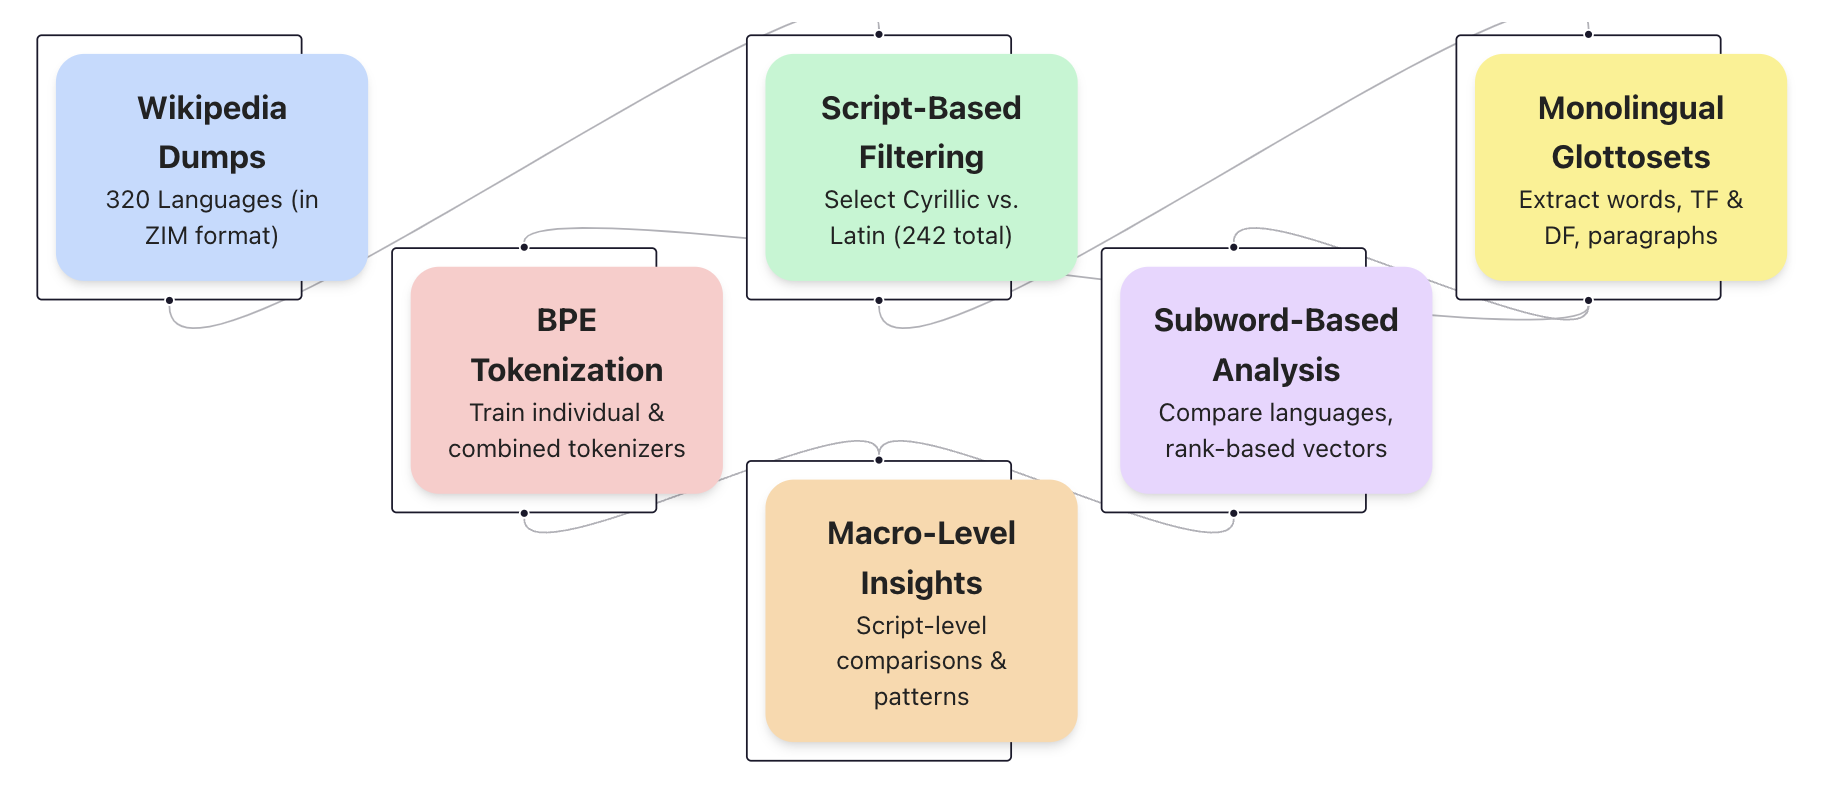
\includegraphics[width=0.9\textwidth]{workflow.png}
  \caption{Pipeline for subword-based comparative linguistics across 242 languages. Wikipedia dumps undergo script-based filtering, glottoset construction (TF/DF metrics), and BPE tokenization (4096-token vocabulary). This modular workflow culminates in rank-based subword vector analysis to extract macro-level morphological and phylogenetic insights at scale.}
  \label{fig:workflow}
\end{figure}

\begin{figure}[ht]
  \centering
  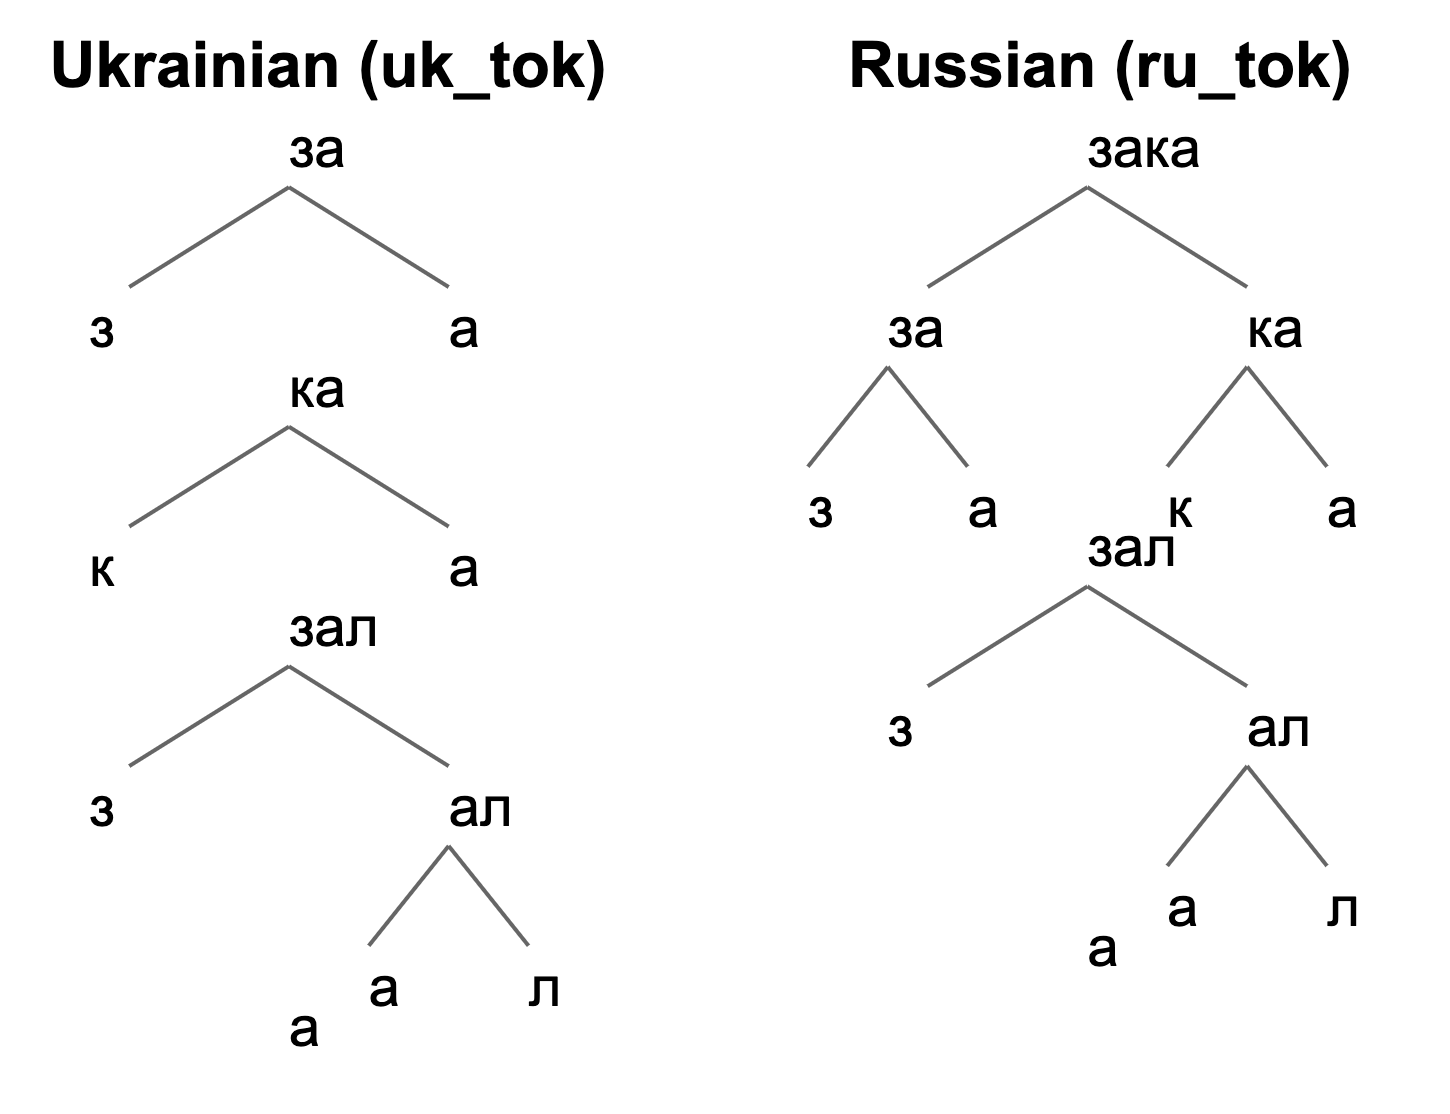
\includegraphics[width=0.6\textwidth]{uk_r_zakazala.png}
  \caption{Hierarchical BPE tokenization trees comparing the word {\fontencoding{T2A}\selectfont заказала} in Ukrainian (left) and Russian (right). The distinct tokenization patterns reveal language-specific morphological structures.}
  \label{fig:bpe_tree}
\end{figure}

\begin{figure}[ht]
  \centering
  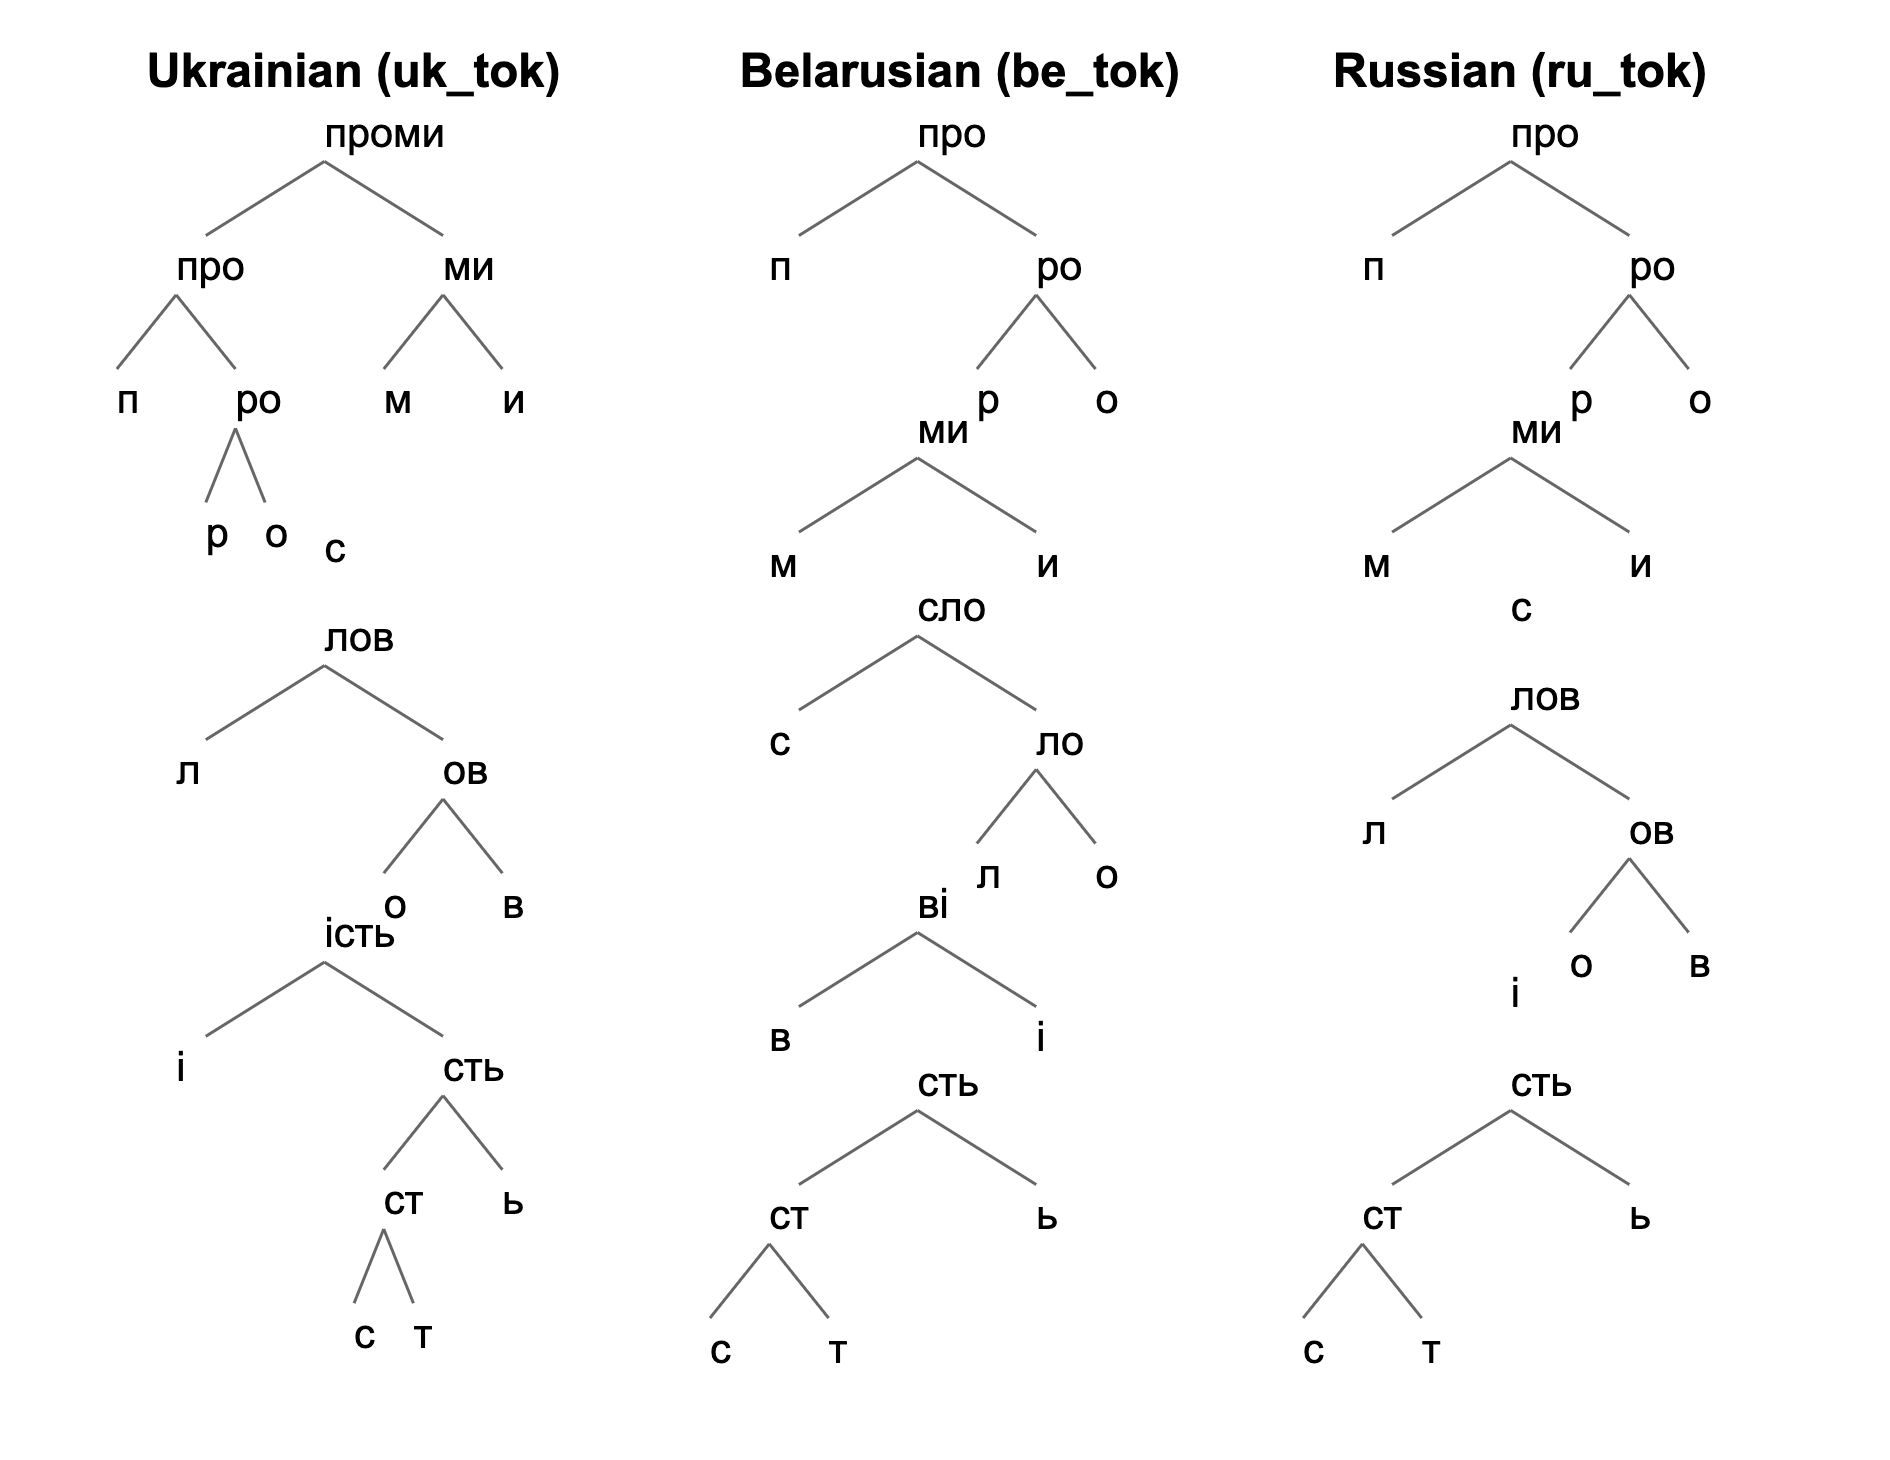
\includegraphics[width=0.8\textwidth]{uk_be_r_promyslovist.png}
  \caption{Hierarchical BPE tokenization trees for the word {\fontencoding{T2A}\selectfont ``промисловість''} (industry) across three East Slavic languages. The Ukrainian tokenization produces semantically consistent morphemes, while Belarusian and Russian models generate more fragmented subword units.}
  \label{fig:bpe_tree2}
\end{figure}

\begin{figure}[ht]
  \centering
  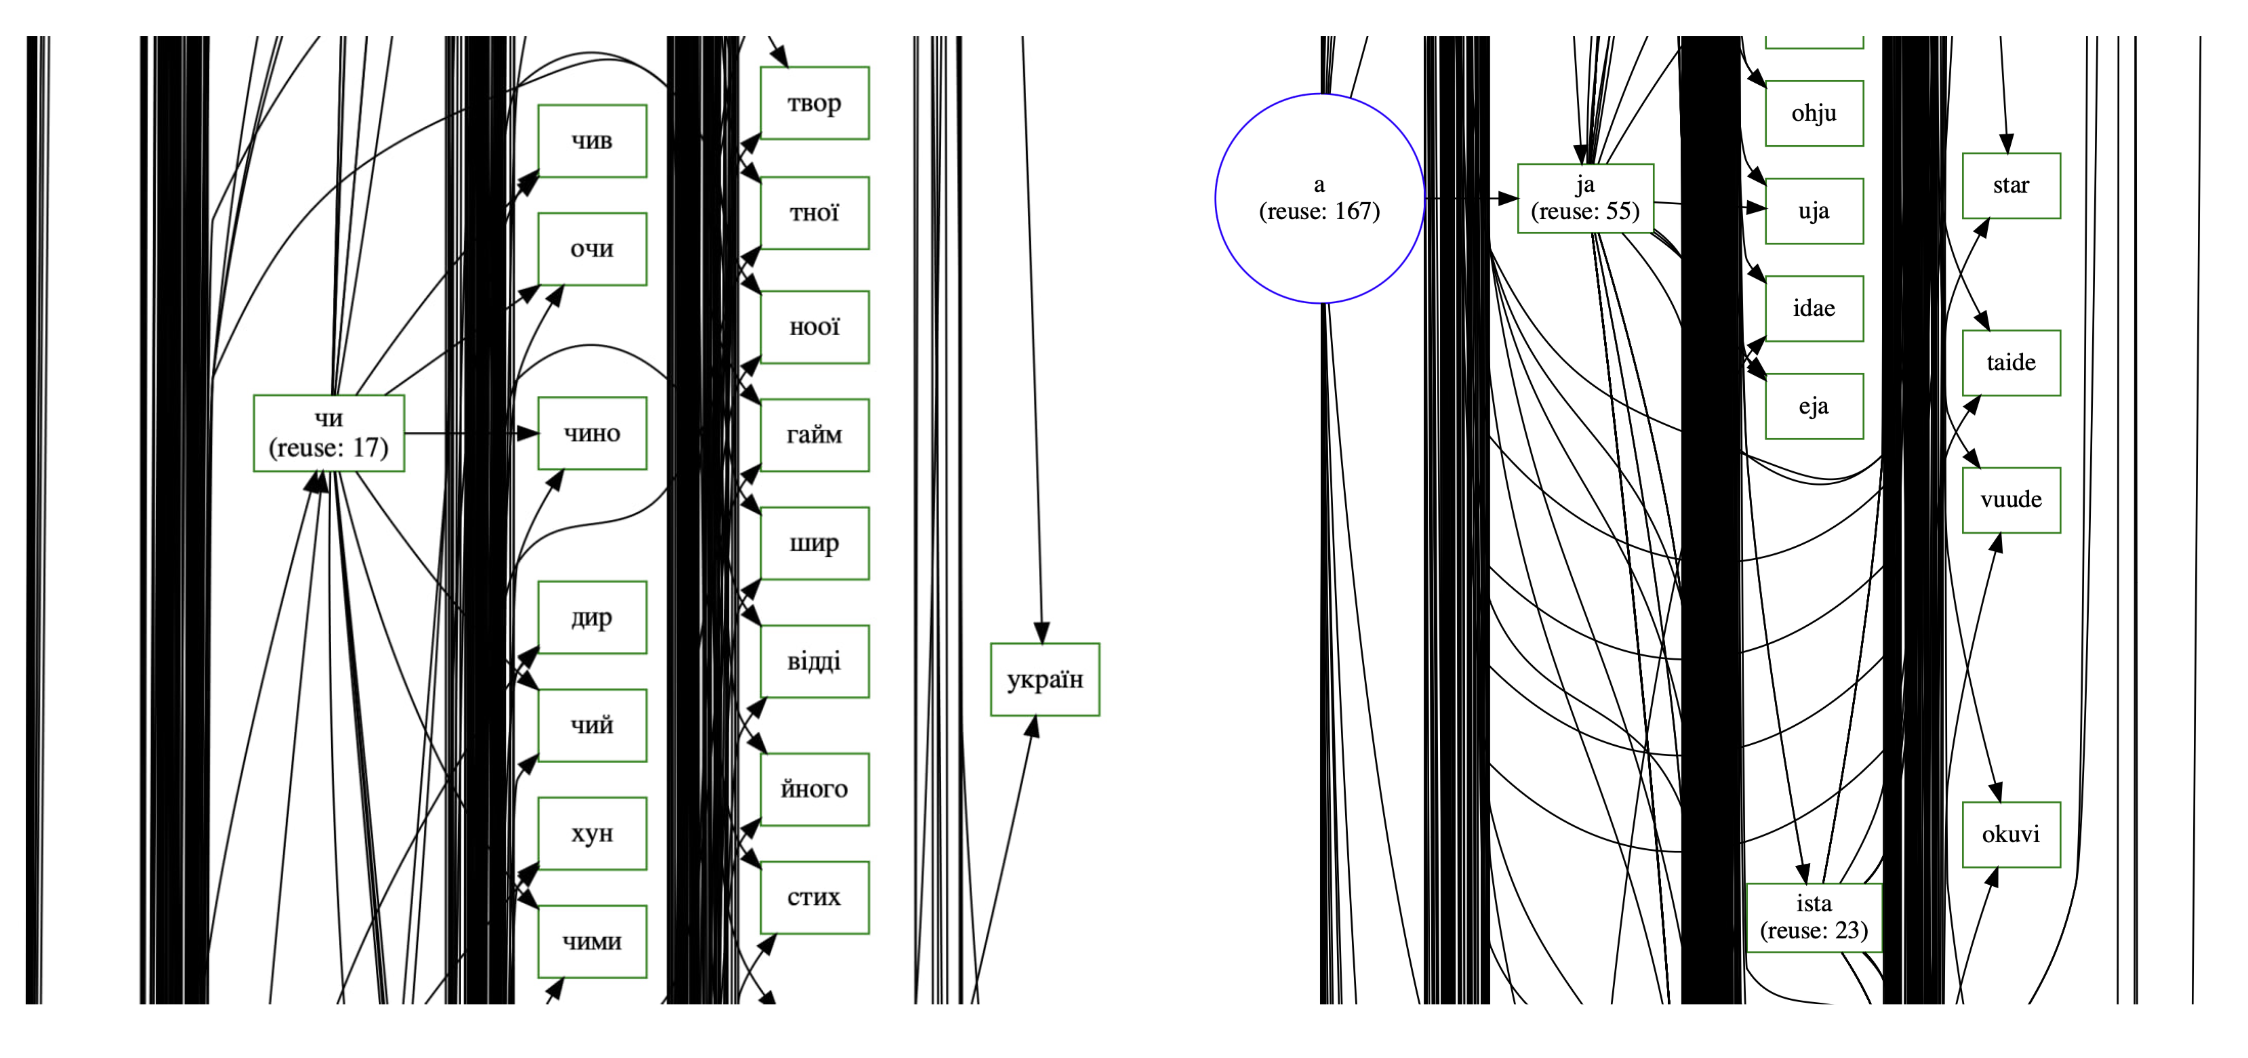
\includegraphics[width=\textwidth]{graph.png}
  \caption{Visualization of interactive BPE merge graphs for Ukrainian (left) and Finnish (right) subword tokenization patterns. The diagrams show directed merge sequences with reuse counts indicated in parentheses. Vertical black bars represent merge steps, while edges show the progression of subword unit formation. The contrasting patterns reflect language-specific morphological characteristics: Ukrainian showing consistent Cyrillic character combinations, while Finnish exhibits agglutinative patterns. Interactive web application available on our repository.}
  \label{fig:bpe_merge}
\end{figure}

\begin{table}[ht]
    \caption{Lexical statistics for a diverse set of languages using Latin and Cyrillic scripts. The table presents vocabulary size (ranging from 1,447 for Cheyenne to 3,207,272 for Hungarian), lexical diversity scores (from 0.009 in Dutch to 0.383 in Cheyenne), median word length (6--10 characters), and top-3 most frequent tokens.}
    \label{tab:lexical_stats_median}
    \centering
    \small
    \renewcommand{\arraystretch}{1.1}
    \begin{tabular}{l c c c c c}
        \toprule
        \textbf{Language} & \textbf{Script} & \textbf{Vocab Size} & \textbf{Lex.\ Div.} & \textbf{Med.\ WL} & \textbf{Top3} \\
        \midrule
        Swiss German & Latin & 565258 & 0.070 & 10 & d, isch, dr \\
        Tajik & Cyrillic & 317780 & 0.041 & 8 & {\fontencoding{T2A}\selectfont дар, аз, ки} \\
        Hungarian & Latin & 3207272 & 0.025 & 10 & a, \'es, az \\
        Lingala & Latin & 23153 & 0.123 & 7 & ya, na, ezal\'i \\
        Zeeuws & Latin & 51177 & 0.087 & 8 & de, n, t \\
        Lak & Cyrillic & 6890 & 0.315 & 7 & {\fontencoding{T2A}\selectfont ва, шагьру, инсан} \\
        Malay & Latin & 637993 & 0.011 & 8 & yang, di, dan \\
        Cheyenne & Latin & 1447 & 0.383 & 6 & ho, e, v\'e \\
        Aymara & Latin & 29323 & 0.171 & 8 & a, jisk, suyu \\
        Friulian & Latin & 44905 & 0.086 & 7 & di, e, al \\
        Javanese & Latin & 281161 & 0.040 & 8 & ing, lan, iku \\
        Rusyn & Cyrillic & 112582 & 0.149 & 8 & {\fontencoding{T2A}\selectfont в, на, є} \\
        Ido & Latin & 129897 & 0.029 & 7 & la, di, e \\
        Norman & Latin & 31509 & 0.106 & 7 & d, est, la \\
        Ligurian & Latin & 133733 & 0.090 & 7 & l, a, de \\
        Karakalpak & Latin & 104775 & 0.144 & 8 & h\'am, menen, bul \\
        Romanian & Latin & 1102965 & 0.013 & 8 & \^in, de, \c{s}i \\
        Somali & Latin & 118361 & 0.076 & 8 & oo, iyo, ka \\
        Lombard & Latin & 239355 & 0.042 & 7 & l, \`e, de \\
        Norwegian Bokm\aa l & Latin & 1918724 & 0.018 & 10 & i, og, en \\
        West Flemish & Latin & 96384 & 0.079 & 8 & de, van, in \\
        M\=aori & Latin & 15232 & 0.033 & 7 & te, ko, o \\
        Icelandic & Latin & 451176 & 0.051 & 10 & \'i, og, \'a \\
        Mongolian & Cyrillic & 235807 & 0.044 & 8 & {\fontencoding{T2A}\selectfont нь, оны, юм} \\
        Dutch & Latin & 2866741 & 0.009 & 10 & de, van, in \\
        Kabyle & Latin & 52338 & 0.106 & 7 & n, d, deg \\
        Tsonga & Latin & 14810 & 0.116 & 8 & hi, na, ya \\
        Madurese & Latin & 33922 & 0.155 & 7 & b\^an, \`e, s\`e \\
        \bottomrule
    \end{tabular}
\end{table}


\begin{table}[ht]
    \caption{Script contamination analysis for languages using non-Latin/non-Cyrillic writing systems. Data shows language names, codes, raw paragraph counts, native script types, and the number of detected Latin and Cyrillic tokens representing potential script contamination.}
    \label{tab:additional_languages}
    \centering
    \small
    \renewcommand{\arraystretch}{1.1}
    \begin{tabular}{l c c c c c}
        \toprule
        \textbf{Lang} & \textbf{Code} & \textbf{Raw pars} & \textbf{Script} & \textbf{Cyrillic} & \textbf{Latin} \\
        \midrule
        Min Nan Chinese & nan & 830227 & Han & 13 & 541415 \\
        Japanese & ja & 12737874 & Japanese & 915 & 298430 \\
        Chinese & zh & 7206035 & Han & 554 & 117304 \\
        Greek & el & 1733250 & Greek & 363 & 96009 \\
        Hebrew & he & 3368324 & Hebrew & 479 & 90907 \\
        Korean & ko & 3333575 & Hangul & 635 & 81612 \\
        Arabic & ar & 4624040 & Arabic & 246 & 58738 \\
        Persian & fa & 3132901 & Arabic & 165 & 51729 \\
        Balinese & ban & 87175 & Balinese & 4 & 48922 \\
        Thai & th & 944565 & Thai & 305 & 43559 \\
        Armenian & hy & 1647293 & Armenian & 2579 & 41259 \\
        Egyptian Arabic & arz & 5166127 & Arabic & 23 & 39349 \\
        Buginese & bug & 36776 & Lontara & 0 & 19834 \\
        Min Dong Chinese & cdo & 28589 & Han & 0 & 19197 \\
        Georgian & ka & 644781 & Georgian & 387 & 15234 \\
        Bengali & bn & 854059 & Bengali & 64 & 13786 \\
        Hindi & hi & 703141 & Devanagari & 80 & 13369 \\
        Tamil & ta & 820809 & Tamil & 28 & 11153 \\
        Hakka Chinese & hak & 14204 & Han & 2 & 10368 \\
        Malayalam & ml & 464433 & Malayalam & 31 & 9848 \\
        Sinhalese & si & 166475 & Sinhala & 3 & 9552 \\
        Burmese & my & 451126 & Burmese & 8 & 9467 \\
        Urdu & ur & 660706 & Arabic & 62 & 9172 \\
        Cantonese & yue & 373575 & Han & 53 & 8418 \\
        South Azerbaijani & azb & 605161 & Arabic & 18 & 7459 \\
        Goan Konkani & gom & 39569 & Devanagari & 0 & 6955 \\
        Marathi & mr & 349639 & Devanagari & 10 & 6842 \\
        Cambodian & km & 99641 & Khmer & 13 & 6324 \\
        Telugu & te & 832028 & Telugu & 3 & 6170 \\
        Tachelhit & shi & 7811 & Tifinagh & 0 & 5799 \\
        \bottomrule
    \end{tabular}
\end{table}








\end{document}
